\documentclass{article}

\usepackage{microtype}
\usepackage{graphicx}
\usepackage{subcaption}
\usepackage{booktabs}
\usepackage{amsmath}
\usepackage{amssymb}
\usepackage{mathtools}
\usepackage{hyperref}
\usepackage{icml2026}
\urlstyle{same}

\newcommand{\thscan}{Th229-ScanBench}
\newcommand{\hz}{\,\mathrm{Hz}}
\newcommand{\anonrepo}{\url{https://anonymous.4open.science/r/th229-scanbench-5218/README.md}}
\graphicspath{{results/figures/}{./}}
\icmltitlerunning{Th229-ScanBench}

\begin{document}

\twocolumn[
  \icmltitle{Th229-ScanBench: A Benchmark for Detection in Sparse, Heteroscedastic Time Series from a Thorium-229 Nuclear Clock}

  \begin{icmlauthorlist}
    \icmlauthor{Anonymous Authors}{anon}
  \end{icmlauthorlist}
  \icmlaffiliation{anon}{Anonymous Institution}
  \icmlcorrespondingauthor{Anonymous Authors}{anonymous@example.com}
  \icmlkeywords{AI for Physics, simulation-based inference, sparse time series, heteroscedastic data, thorium-229}

  \vskip 0.3in
]
\printAffiliationsAndNotice{}

\begin{abstract}
\thscan{} is a public benchmark for binary detection in sparse, irregular, heteroscedastic time series from precision physics, built on 55 temperature-corrected peak-b measurements from the JILA scan-level thorium-229 nuclear-clock record. The primary task fixes the observed timestamps, crystal identities, and uncertainties while injecting controlled sinusoidal frequency shifts, yielding 6,336 labeled examples on a fixed train/validation/test split. The strongest baseline is amortized simulation-based inference with a continuous log-uniform amplitude prior and bounded posterior reparameterization (AUROC 0.793, AP 0.846), matching or narrowly exceeding a hierarchical sinusoid model (0.774, 0.827) and a small Transformer trained on the supervised split (0.769, 0.829). Learned null-model diagnostics show that the X2-only observed-series anomaly remains significant under parametric, Gaussian-mixture, and conditional-flow nulls, so we treat it as a robust data property rather than a detection claim. A damped-sinusoid stress test exposes a cadence ceiling: at small damping times all baselines collapse to chance, while at \(\tau=180\) days SBI and the hierarchical model are most robust to signal-family mismatch. The benchmark, code, fixed splits, and baseline checkpoints are released for reproducible method comparison.
\end{abstract}

\section{Introduction}

Precision spectroscopy increasingly produces time-domain data that look unlike standard machine-learning benchmarks: the records are short, irregularly sampled, heteroscedastic, and tied to nuisance metadata such as instrument state or sample identity.  The public scan-level thorium-229 frequency-reproducibility record from JILA is a compact example of this regime~\citep{ooi2026frequency,ooi2025zenodo}.  It is far too small for unconstrained large-scale supervised learning, but it is large enough to define a realistic detection benchmark in which the cadence, uncertainties, crystal labels, and temperature metadata are fixed by experiment rather than simulated from a convenient grid.

\thscan{} turns this record into an AI benchmark for weak-signal detection in precision physics.  Each input is a length-55 residual-frequency vector on the observed peak-b timestamps.  Labels are created by adding or not adding a controlled time-dependent frequency shift to residual draws from a training-fit, crystal-aware null model.  The benchmark is therefore not a claim about the observed JILA series.  Its purpose is methodological: compare physics-informed periodogram methods, simulator-trained inference, and supervised ML baselines under a leakage-controlled protocol on a sparse real cadence.

The main results are threefold.  First, simulation-based inference (SBI) with neural posterior estimation is the strongest primary-task baseline after careful prior parameterization, reaching AUROC 0.793.  Second, supervised neural sequence models trained on the 1,848 training examples are competitive but do not exceed SBI; the best Transformer reaches AUROC 0.769.  Third, a damped-sinusoid stress test exposes signal-family mismatch: methods trained or designed for persistent sinusoids lose substantial AUROC when the signal decays before most observations.  These outcomes make the benchmark useful not only as a leaderboard, but as a controlled testbed for data efficiency, prior specification, and robustness to physically motivated distribution shift.

This work targets two themes the AI4Physics community has identified as underserved: dataset-building in physics areas where public records are sparse, and likelihood-free inference on small, structured precision-physics data.  \thscan{} provides a leakage-controlled testbed for both.  An anonymous release is available at \anonrepo{}.

\section{Related Work}

\paragraph{Simulation-based inference in physics.}
Simulation-based inference (SBI) replaces an explicit likelihood with samples from a forward simulator and has become a standard tool for physics settings where the simulator is available but the likelihood is not~\citep{cranmer2020frontier}.  Neural posterior estimation (NPE) methods learn amortized approximations to \(p(\theta\mid x)\) using conditional density estimators~\citep{papamakarios2016fast}; SNPE-C and automatic posterior transformation extend this idea to sequential proposals and flow-based posteriors~\citep{greenberg2019automatic}.  Community benchmarks such as \citet{lueckmann2021benchmarking} have clarified where SBI methods succeed and fail, but most examples are generic simulators or larger scientific problems rather than small precision-spectroscopy records.  \thscan{} focuses on a complementary regime: a fixed real cadence with only 55 observation times, structured uncertainties, and a null model that can itself be audited.

\paragraph{Software and density estimation.}
Our SBI baseline uses the sbi package~\citep{tejero2020sbi}, which provides implementations of SNPE-style inference methods and neural density estimators.  The v2 posterior uses neural spline flows~\citep{durkan2019neural}, chosen because they can represent non-Gaussian marginal posteriors while remaining cheap enough for a reproducible workshop benchmark.  The learned-null diagnostic also uses a conditional spline flow, but Section~\ref{sec:nulls} shows that additional flexibility is not automatically beneficial when the observation-level training set is small.

\paragraph{Physics time-series benchmarks.}
Physics ML benchmarks often emphasize large-sample regimes, such as collider anomaly challenges or astronomical classification tasks.  PLAsTiCC, for example, evaluates classification of simulated LSST-like transient time series at much larger scale~\citep{kessler2019plasticc}.  Such benchmarks are valuable, but they do not isolate the sparse-cadence, heteroscedastic, real-metadata regime common in precision measurements.  The thorium-229 nuclear transition also has independent motivation for searches for ultralight dark matter and other slowly varying effects~\citep{fuchs2025searching}, but translating Hz-scale amplitude limits into coupling constraints is model-dependent and outside the scope of this benchmark.

\section{Data and Benchmark Protocol}

The source record contains scan-level line measurements for \(^{229}\mathrm{Th}:\mathrm{CaF}_2\).  We use the canonical 73-row published scan-level subset and select the 55 peak-b rows as the primary task because peak b is the lower-temperature-sensitivity line in the JILA analysis.  The 55 rows span 487.73 days and contain 15 C10, 12 C13, and 28 X2 measurements.  We fit the temperature trend using the canonical C10 and C13 records, subtract it, and remove a target-peak weighted mean offset.  Details of the 72-row literal readme rule versus the 73-row canonical scan-key rule are deferred to Appendix~\ref{app:subset}; both choices give the same 55 peak-b rows.

A benchmark example is a residual vector \(x\in\mathbb{R}^{55}\).  Null examples are sampled from the selected null model, a Gaussian model with crystal-specific extra variance and an X2-only Gaussian outlier component fitted only on the observation-level null-training subset.  Signal examples add
\begin{equation}
  \delta\nu(t) = A\cos(2\pi f t + \phi)
\end{equation}
at the same 55 timestamps.  We use 12 periods from 7 to 365 days and 11 amplitudes from 100 to 6500 Hz.  For each period-amplitude cell, we use 24 phases and both labels, giving 6,336 examples.  Splits are fixed by phase index within every cell: 14 phases for training, 5 for validation, and 5 for test, or 1,848/660/660 examples per class.  Detection thresholds are always calibrated from validation null examples only.

\section{Baselines}

\paragraph{Sinusoid-search baselines.}
Weighted harmonic regression fits a sinusoid at each searched frequency with uncertainty weights and crystal-specific offsets.  Generalized Lomb--Scargle uses the same weighted search with a single global offset~\citep{lomb1976least,scargle1982studies,zechmeister2009generalised}.  The hierarchical sinusoid model uses a shared sinusoid with crystal-specific offsets and the selected null-model uncertainty scale.  These methods fit per example and do not use benchmark labels for training.

\paragraph{Supervised baselines.}
The random forest is trained on the fixed training split using periodogram powers at the 12 benchmark periods and seven summary statistics.  The neural sequence baselines take length-55 sequences with eight channels per timestep: z-scored residual frequency, z-scored frequency uncertainty, z-scored temperature, three crystal one-hot channels, normalized time since first observation, and a constant channel.  The 1D CNN has three residual convolution blocks with kernel size 5 and channel widths \(32,64,64\), layer normalization, global average pooling, and a two-layer MLP head, for 39,105 trainable parameters.  The Transformer uses a learned CLS token, learned length-56 positional embedding, model dimension 64, two encoder layers, four attention heads, feed-forward width 128, and a two-layer MLP head, for 75,521 parameters.  Both models use binary cross-entropy, AdamW, batch size 256, a grid over learning rates \(\{10^{-3},3\times10^{-4},10^{-4}\}\) and weight decays \(\{0,10^{-4}\}\), at most 200 epochs, and early stopping with patience 20 on validation AUROC.  We run one seeded grid per architecture; validation data select hyperparameters and calibrate thresholds, but never update weights.

\paragraph{Simulation-based inference.}
The SBI baseline uses neural posterior estimation (SNPE-C/NPE) with a neural spline flow density estimator from the sbi package.  The simulator samples \(A\), log-period, and phase, evaluates the sinusoid on the 55 real timestamps, and adds a draw from the same training-fit parametric null model.  The v2 training run uses 100,000 simulator draws, a neural spline flow with four transforms, hidden width 64, eight spline bins, batch size 512, and 12 training epochs; the recorded training time is 517 seconds on the local accelerator.  The score is posterior mass \(p(A>50\hz\mid x)\), marginalizing over period and phase using 256 posterior samples per example.  A first version used a point mass at \(A=0\) and unbounded posterior coordinates; it reached AUROC 0.728 and placed 17\% of amplitude samples outside the physical \([0,6500]\hz\) box.  The headline v2 model replaces this with a continuous log-uniform amplitude prior on \([1,6500]\hz\) and bounded logit reparameterizations for amplitude, log-period, and phase.  This reduces the physical-support diagnostic to 0\% and improves AUROC to 0.793.

\section{Primary Results}

\begin{table*}[t]
  \centering
  \small
  \setlength{\tabcolsep}{6pt}
  \caption{Primary test-set detection metrics with 95\% bootstrap confidence intervals from 1,000 resamples of the 1,320 held-out test examples.  SBI v2 has the best point estimates, but its AUROC interval overlaps the hierarchical and Transformer intervals.}
  \label{tab:main}
  \begin{tabular}{lccc}
    \toprule
    Method & AUROC (95\% CI) & AP (95\% CI) & Test FPR \\
    \midrule
    Weighted harmonic & 0.700 (0.673, 0.725) & 0.748 (0.717, 0.777) & 0.050 \\
    GLS & 0.724 (0.696, 0.751) & 0.776 (0.749, 0.802) & 0.050 \\
    Hierarchical sinusoid & 0.774 (0.748, 0.797) & 0.827 (0.802, 0.848) & 0.042 \\
    Random forest & 0.712 (0.686, 0.741) & 0.769 (0.742, 0.797) & 0.070 \\
    SBI NPE v2 & \textbf{0.793} (0.769, 0.815) & \textbf{0.846} (0.825, 0.866) & 0.035 \\
    Neural CNN & 0.758 (0.732, 0.784) & 0.817 (0.794, 0.839) & 0.042 \\
    Neural Transformer & 0.769 (0.743, 0.796) & 0.829 (0.806, 0.852) & 0.050 \\
    \bottomrule
  \end{tabular}
\end{table*}

\begin{table}[t]
  \centering
  \footnotesize
  \setlength{\tabcolsep}{3.3pt}
  \caption{Representative-period performance.  At 30 days, SBI and the hierarchical model are strongest; at 180 days, SBI has the lowest \(A_{95}\) among reported baselines.}
  \label{tab:representative}
  \begin{tabular}{llccc}
    \toprule
    Method & \(P\) & AUROC & AP & \(A_{95}\) Hz \\
    \midrule
    Hierarchical & 30 d & 0.825 & 0.651 & 969 (938--979) \\
    SBI NPE v2 & 30 d & 0.827 & 0.669 & 1458 (1375--1469) \\
    Transformer & 30 d & 0.774 & 0.584 & 1458 (1438--1469) \\
    Random forest & 30 d & 0.781 & 0.513 & 2112 (2025--2144) \\
    \midrule
    Hierarchical & 180 d & 0.727 & 0.449 & 2950 (2156--3075) \\
    SBI NPE v2 & 180 d & 0.838 & 0.665 & 979 (969--984) \\
    Transformer & 180 d & 0.786 & 0.601 & 2112 (984--2142) \\
    Random forest & 180 d & 0.689 & 0.331 & 3138 (3117--3150) \\
    \bottomrule
  \end{tabular}
\end{table}

The overall ranking in Table~\ref{tab:main} separates method families while showing that the top intervals overlap.  The physics-informed hierarchical sinusoid model remains strong, and the simulator-trained SBI v2 baseline has the highest point estimates in both AUROC and AP.  The Transformer nearly matches the hierarchical model in overall AUROC and slightly exceeds it in AP, but it does not exceed SBI v2.  The random forest remains a useful low-capacity supervised baseline, below the neural sequence models and hierarchical model but close to the simpler periodogram methods.

The performance gap between SBI v2 (AUROC 0.793) and the supervised neural baselines (Transformer 0.769, CNN 0.758) is consistent with the simulation-budget asymmetry.  SBI trains on 100,000 simulator draws using the same parametric null family that generates the benchmark examples, while the supervised models train on 1,848 labeled training examples without simulator access.  The gap therefore measures how much simulator availability is worth on this benchmark scale, not an intrinsic ranking of neural architectures.  A natural follow-up is to train supervised models on simulator-augmented data; we leave that variant to future work.

\begin{figure}[t]
  \centering
  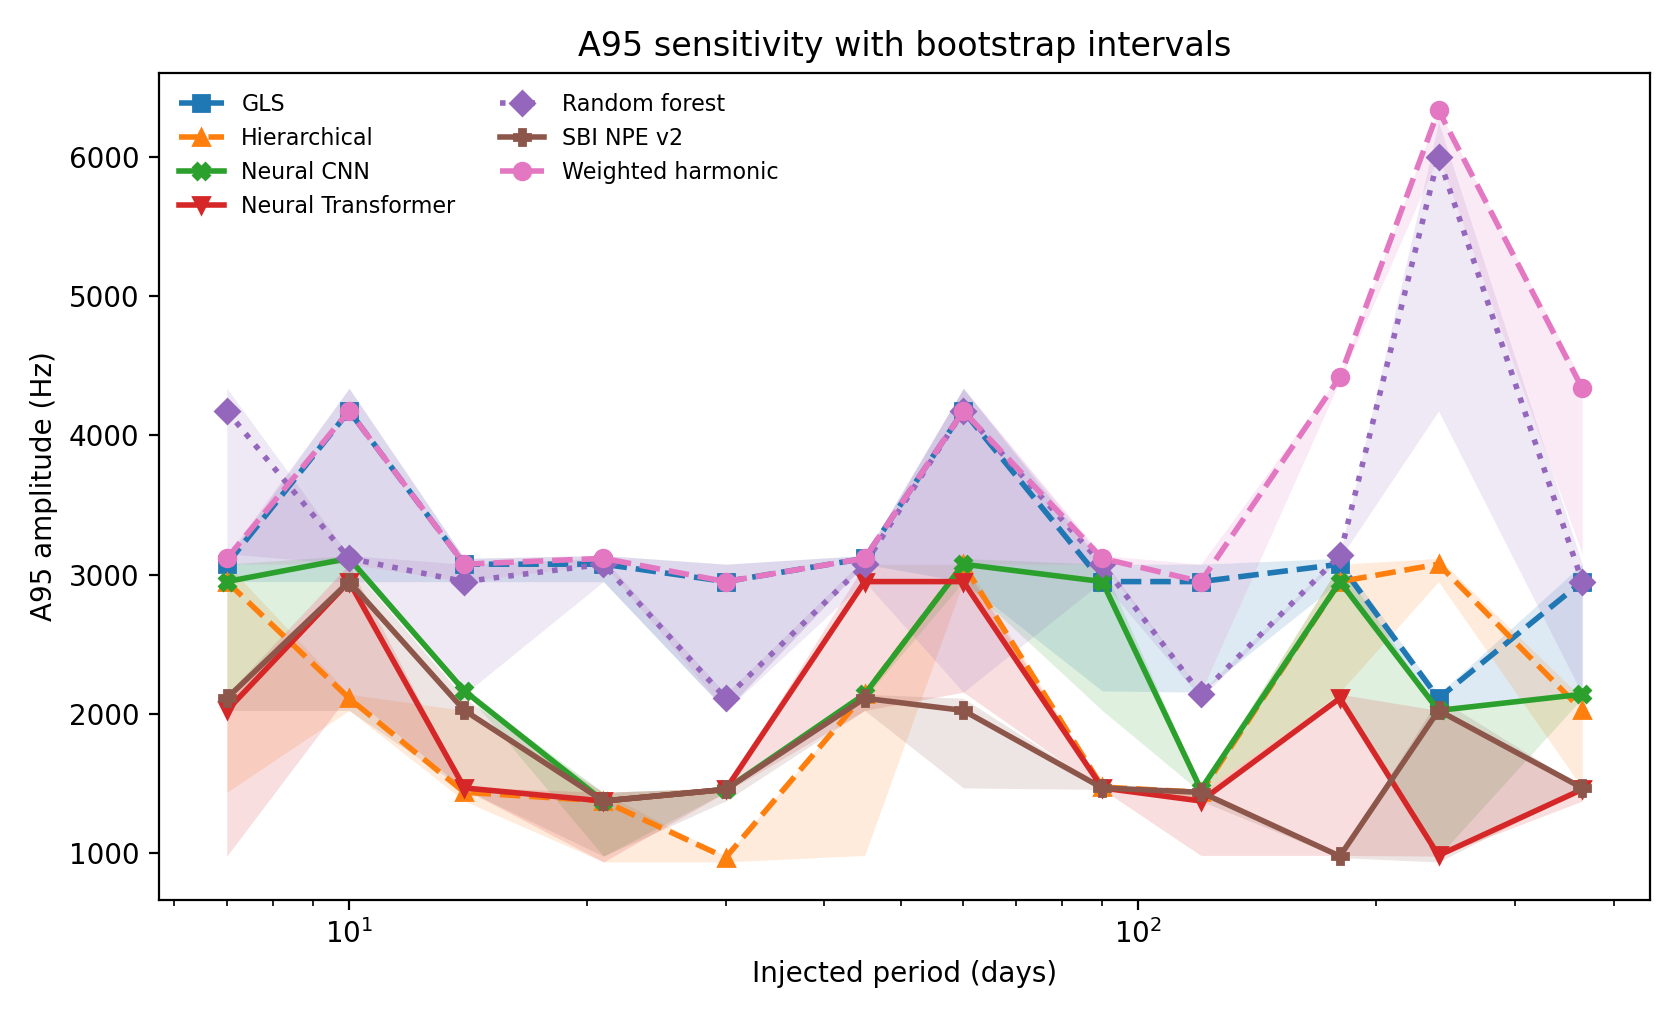
\includegraphics[width=\columnwidth]{final_a95_vs_frequency_with_uncertainty.png}
  \caption{\(A_{95}\) sensitivity curves across injected period, with shaded 16--84\% bootstrap intervals from validation-threshold and test-phase resampling.  Sensitivity varies strongly with period and method: SBI v2 and the hierarchical model give the lowest \(A_{95}\) in different parts of the grid.}
  \label{fig:a95}
\end{figure}

The \(A_{95}\) curves in Figure~\ref{fig:a95} show that no method dominates uniformly.  The hierarchical model is most sensitive at 30 days, with \(A_{95}=969\hz\).  SBI v2 is strongest at 180 days among the representative rows, with \(A_{95}=979\hz\).  Because \(A_{95}\) is calibrated from validation null examples and resamples only validation thresholds and test phases, these intervals should be read as benchmark uncertainty rather than uncertainty in the original JILA frequency measurements.

\section{Null-Model Diagnostics}\label{sec:nulls}

We use the observed JILA residual series only as a diagnostic for null calibration.  Under the parametric null, the all-peak-b series has empirical p-value 0.659 and the C10+C13 subset has p-value 0.922.  The X2-only subset is significant under all tested nulls: p-value 0.00585 for the parametric X2-mixture null, 0.00195 for a crystal-specific Gaussian mixture, and 0.00195 for a conditional spline flow.  Held-out log likelihood favors the parametric null, with mean validation log likelihood \(-9.12\), compared with \(-9.41\) for the GMM and \(-15.34\) for the conditional flow.  The poor held-out likelihood of the conditional flow propagates downstream: an SBI variant trained with the learned-flow null (Appendix~\ref{app:sbi-versions}) collapses to AUROC 0.456, confirming that simulator quality dominates baseline performance at this dataset size.  We therefore view the X2 anomaly as a robust property of the observed data, not an artifact removed by a more flexible null model and not a signal claim.

\begin{figure}[t]
  \centering
  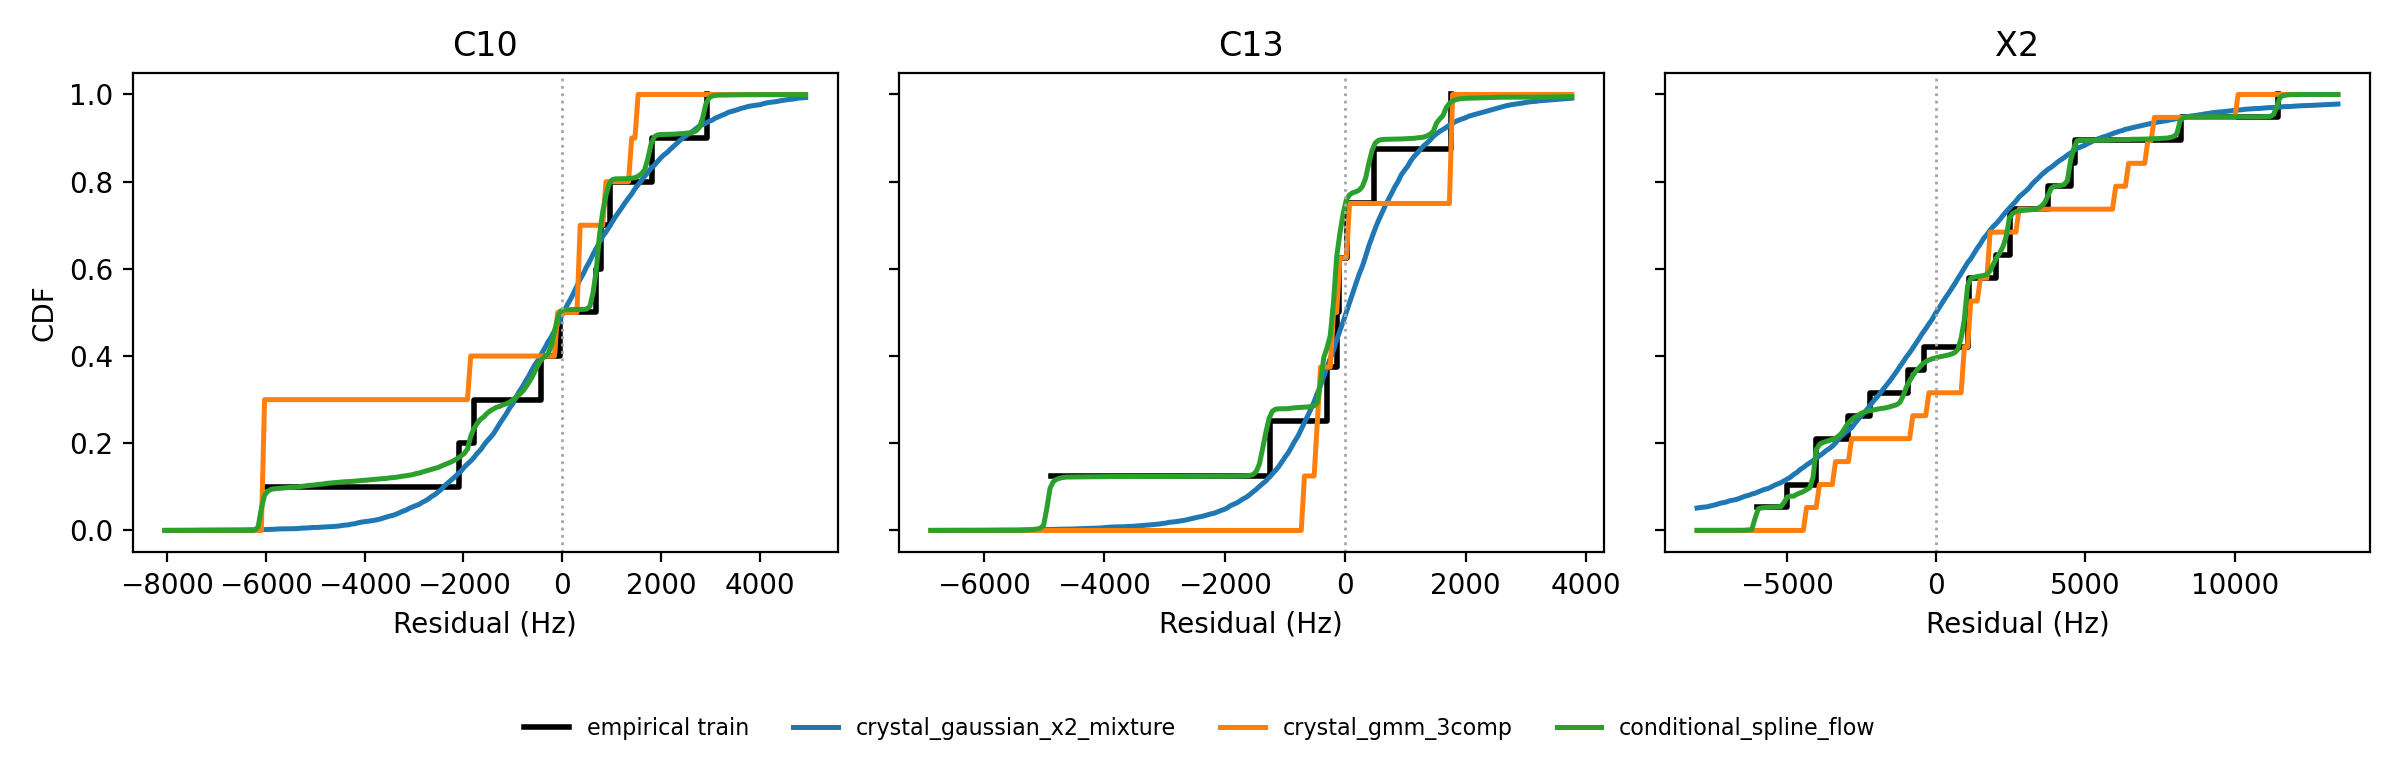
\includegraphics[width=\columnwidth]{null_model_calibration_by_crystal.png}
  \caption{Per-crystal empirical training CDFs are overlaid with parametric, GMM, and conditional-flow null CDFs; vertical dotted lines mark zero residual.  Learned nulls do not explain away the X2 tail behavior, and the conditional flow fits the small training split poorly by held-out likelihood.}
  \label{fig:nulls}
\end{figure}

\section{Damped-Sinusoid Stress Test}

To test whether \thscan{} can support more than one signal family, we add a zero-shot damped-sinusoid task,
\begin{equation}
  \delta\nu(t) = A\exp(-t/\tau)\cos(2\pi f t + \phi),
\end{equation}
with \(\tau\in\{30,90,180\}\) days and the same period, amplitude, phase, split, and null protocols as the main benchmark.  No baseline is retrained.  Validation null examples are used only to recalibrate the 5\% threshold for each stress-test family.

\begin{figure}[t]
  \centering
  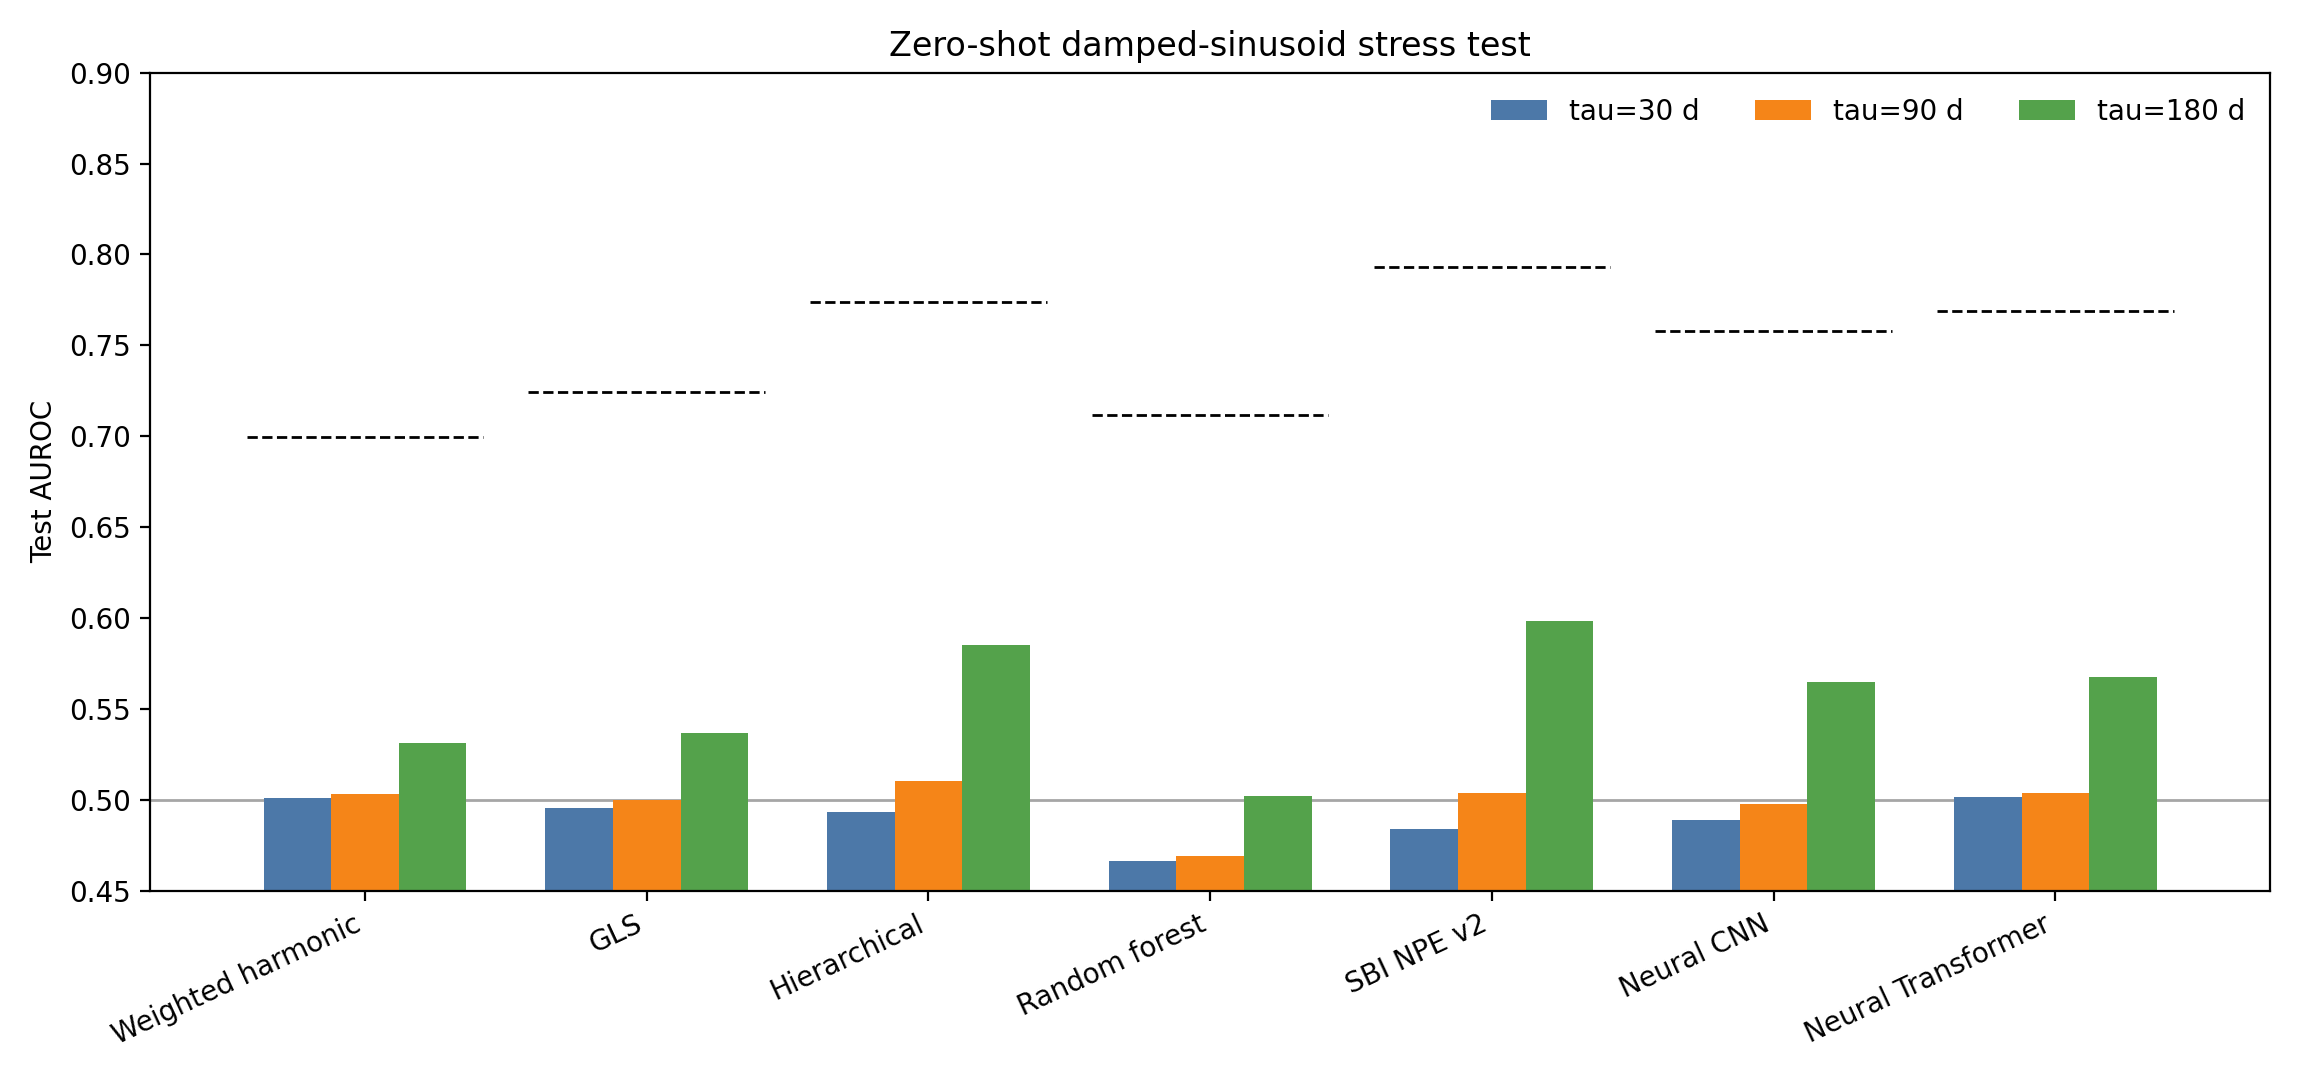
\includegraphics[width=\columnwidth]{stress_damped_auroc_degradation.png}
  \caption{Zero-shot damped-sinusoid stress test. Bars show test AUROC at three damping times \(\tau\); dashed horizontal lines mark each baseline's main-benchmark AUROC for reference. At \(\tau \le 90\) days all methods collapse to chance because the signal decays before most observations; at \(\tau = 180\) days, SBI v2 (0.598) and the hierarchical sinusoid model (0.585) are most robust to signal-family mismatch.}
  \label{fig:stress}
\end{figure}

The stress test in Figure~\ref{fig:stress} shows a limitation of the cadence as much as a limitation of the methods.  At \(\tau=30\) days over a 487.73-day record, the damped signal decays by a factor of approximately \(10^{-7}\) across the observation window; effectively, fewer than five of the 55 timestamps see meaningful signal amplitude regardless of \(A\).  The simultaneous failure of all baselines at \(\tau \le 90\) days reflects this cadence-imposed ceiling rather than a method comparison.  At \(\tau=180\) days, SBI v2 is most robust (AUROC 0.598), followed by the hierarchical sinusoid model (0.585), the Transformer (0.568), the CNN (0.565), generalized Lomb--Scargle (0.537), weighted harmonic regression (0.531), and the random forest (0.502).  This suggests that the benchmark can expose signal-family mismatch without changing the measured metadata or the evaluation protocol.

\section{Limitations and Release}

\thscan{} is intentionally small.  It is not a benchmark for training large sequence models from scratch, nor does it use photon-count or lineshape arrays.  Injected amplitudes are reported in Hz; translating them into coupling constraints requires model-specific assumptions.  The null model is trained on only a small observation-level subset, and the X2 diagnostics show that part of the measured record remains difficult to calibrate.  These limitations are part of the benchmark's role: it is a controlled sparse-cadence testbed, not a replacement for future long-duration thorium clock records.

The reusable part of the resource is the separation between fixed experimental metadata and injected signal family.  Future work can keep the same 55 timestamps, crystals, uncertainties, and split rules while adding alternative signal morphologies or cleaner subsets.  The curated dataset, benchmark generation code, baseline implementations, trained checkpoints, and evaluation scripts are available anonymously at \anonrepo{}; source JILA data follow CC BY 4.0 and benchmark code is MIT licensed.

\section*{Impact Statement}

This work provides a benchmark for method development in precision-physics time series.  The main risk is overinterpreting synthetic-injection performance or observed-series diagnostics as evidence for new physics.  We mitigate this by fixing leakage-controlled splits, reporting null diagnostics separately from benchmark metrics, and explicitly treating the X2-only observed-series anomaly as a calibration/data-property result rather than a detection claim.  By releasing fixed splits, leakage tests, and trained-checkpoint registries, the benchmark supports reproducible methodological development in precision-physics machine learning, lowering the barrier for ML researchers to engage with this class of physics problems.

\bibliography{main_paper}
\bibliographystyle{icml2026}

\appendix

\section{Subset Reconciliation}\label{app:subset}

The source CSV has 428 rows because scans appear with several correction and fit choices.  The readme states that the published subset uses Lorentzian fits with the mem int correction, except that the earliest X2 rows use memory-corrected Lorentzians because no intensity data were available.  Applying this rule literally gives 72 rows.  The CSV and folder inventory contain 73 unique Lorentzian scan keys, matching the JILA paper's 73 line scans; the extra row is a 2024-09-25 X2 peak-c scan with mem but no mem int.  We use the canonical 73-row scan-level subset and record both rules in the released audit table.  The primary peak-b count is 55 under both choices, so the benchmark examples and all reported numbers are unaffected by this reconciliation.

\section{Dataset Card}\label{app:dataset-card}

Table~\ref{tab:dataset-card} summarizes the fixed example counts used by the main sinusoid task.  The split columns count null and injected examples after expanding the 12-period, 11-amplitude, 24-phase grid.  Splits are stratified by phase index within every period-amplitude cell, so each cell contributes the same number of train, validation, and test phases.  Stress-test datasets use the same schema and split rule, but replace only the injected signal family.

\begin{table}[h!]
  \centering
  \footnotesize
  \caption{Fixed split sizes for the primary sinusoid benchmark.}
  \label{tab:dataset-card}
  \begin{tabular}{lrrr}
    \toprule
    Split & Null & Injected & Total \\
    \midrule
    Train & 1848 & 1848 & 3696 \\
    Validation & 660 & 660 & 1320 \\
    Test & 660 & 660 & 1320 \\
    \bottomrule
  \end{tabular}
\end{table}

\section{SBI Version Comparison}\label{app:sbi-versions}

The SBI variants isolate two implementation lessons.  The v1 model used a discrete-continuous mixture prior on amplitude, which a continuous neural spline flow cannot model cleanly in unconstrained coordinates.  Replacing that prior with a continuous log-uniform amplitude prior under bounded reparameterization eliminates the support diagnostic and improves the primary-task point estimate.  The v3 model keeps the v2 parameterization but substitutes the parametric null with the learned conditional-flow null, confirming that the overfitting diagnosed in Section~\ref{sec:nulls} propagates into downstream SBI performance.

\begin{table}[h!]
  \centering
  \scriptsize
  \caption{SBI prior/noise variants.  The headline model is v2; v3 uses the learned-flow null and is a negative result.  The OOP column is the stricter any-axis prior-support median; the v1 amplitude-only physical-box diagnostic was 17\%.}
  \label{tab:sbi-versions}
  \begin{tabular}{lcccc}
    \toprule
    Version & AUROC & AP & FPR & OOP \\
    \midrule
    v1 & 0.728 & 0.787 & 0.058 & 0.504 \\
    v2 & 0.793 & 0.846 & 0.035 & 0.000 \\
    v3 & 0.456 & 0.476 & 0.245 & 0.000 \\
    \bottomrule
  \end{tabular}
\end{table}

\section{Stress-Test Summary}

All stress-test evaluations are zero-shot: no supervised model is retrained, no SBI posterior is retrained, and the periodogram-style baselines keep their persistent-sinusoid templates.  Thresholds are recalibrated separately for each stress-test family using validation null examples only.  The \(\tau=180\)-day column is the most informative cross-method comparison, because the \(\tau=30\) and \(\tau=90\)-day rows are dominated by the cadence ceiling described in the main text.

\begin{table}[h!]
  \centering
  \scriptsize
  \setlength{\tabcolsep}{3pt}
  \caption{Zero-shot damped-sinusoid AUROC by damping time.  Values are from the stress-test test split; deltas relative to the main benchmark are omitted here for compactness.}
  \begin{tabular}{lccc}
    \toprule
    Method & \(\tau=30\) d & \(\tau=90\) d & \(\tau=180\) d \\
    \midrule
    Weighted harmonic & 0.501 & 0.503 & 0.531 \\
    GLS & 0.496 & 0.500 & 0.537 \\
    Hierarchical sinusoid & 0.493 & 0.510 & 0.585 \\
    Random forest & 0.466 & 0.469 & 0.502 \\
    SBI NPE v2 & 0.484 & 0.504 & 0.598 \\
    Neural CNN & 0.489 & 0.498 & 0.565 \\
    Neural Transformer & 0.501 & 0.504 & 0.568 \\
    \bottomrule
  \end{tabular}
\end{table}

\section{Bootstrap and Null Diagnostic Details}

The headline AUROC and AP intervals in Table~\ref{tab:main} are computed by resampling the 1,320 test examples with replacement for 1,000 bootstrap replicates using a fixed seed.  This preserves the already-frozen predictions and therefore does not change any baseline score, threshold, or trained checkpoint.  The resulting table is saved as results/tables/headline\_metrics\_with\_ci.csv in the release.  The null-model diagnostics in Table~\ref{tab:null-appendix} report the X2-only p-value and validation held-out log likelihood side by side, emphasizing that the more flexible conditional flow does not improve held-out calibration.

\begin{table}[h!]
  \centering
  \scriptsize
  \setlength{\tabcolsep}{4pt}
  \caption{Observed X2-only p-values and validation held-out log likelihood by null model.}
  \label{tab:null-appendix}
  \begin{tabular}{lcc}
    \toprule
    Null model & X2 p-value & Held-out LL \\
    \midrule
    Parametric X2 mixture & 0.00585 & \(-9.12\) \\
    Crystal GMM & 0.00195 & \(-9.41\) \\
    Conditional flow & 0.00195 & \(-15.34\) \\
    \bottomrule
  \end{tabular}
\end{table}

\end{document}
